\documentclass[12pt]{beamer}

\usetheme{Oxygen}
\usepackage{thumbpdf}
\usepackage{wasysym}
%\usepackage{ucs}
\usepackage[utf8]{inputenc}
\usepackage{pgf,pgfarrows,pgfnodes,pgfautomata,pgfheaps,pgfshade}
\usepackage{verbatim}

\pdfinfo
{
  /Title       (A practical Introduction to Lattice Boltzmann Method)
  /Creator     (Institute of Applied Mechanics)
  /Author      (Manuel Diaz)
}


\title{Lattice Boltzmann Method}
\subtitle{A practical Introduction}
\author{Manuel Diaz}
%\date{May 23th 2012}

\begin{document}

\frame{\titlepage}

\section*{}
\begin{frame}
  \frametitle{Outline}
  \tableofcontents[section=1,hidesubsections]
\end{frame}

\AtBeginSection[]
{
  \frame<handout:0>
  {
    \frametitle{Outline}
    \tableofcontents[currentsection,hideallsubsections]
  }
}

\AtBeginSubsection[]
{
  \frame<handout:0>
  {
    \frametitle{Outline}
    \tableofcontents[sectionstyle=show/hide,subsectionstyle=show/shaded/hide]
  }
}

\newcommand<>{\highlighton}[1]{%
  \alt#2{\structure{#1}}{{#1}}
}

\newcommand{\icon}[1]{\pgfimage[height=1em]{#1}}



%%%%%%%%%%%%%%%%%%%%%%%%%%%%%%%%%%%%%%%%%
%%%%%%%%%% Content starts here %%%%%%%%%%
%%%%%%%%%%%%%%%%%%%%%%%%%%%%%%%%%%%%%%%%%



\section{Introduction}

\begin{frame}
  \frametitle{Introduction}
  \framesubtitle{What is the Lattice Boltzmann method?}
  In a nutshell:
  \\
  \alert{``Is a way to simulate fluid flow and energy transfer on a discrete grid 
  by using the Boltzmann transport equation at the messoscopic level rather 
  using the macroscopic continuum level like the Navier-Stokes equations.''}
  \\
  We do this by expressing the fluid in terms of the probabilistic motion 
  of individual particles (effectivebly, in terms of motion of number densities)
  under the various macroscopic forces and microscopic interparticle interaction
  of the forces present in the system.
  
\end{frame}

\begin{frame}
  \frametitle{Introduction}
  \framesubtitle{Setting the perspective}
  Particles commonly are conceptualized as individual molecules which can have interaction with:
    \begin{itemize}
     \item Macroscopic Forces: Gravety, Big Electromagnetic sources.
     \item Microscopic Forces: Electromagnetic interactions between particles
    \end{itemize}
\end{frame}

\begin{frame}
  \frametitle{Introduction}
  \framesubtitle{Setting the right perspective}  
   
  we start by defining a function, $f(\vec{x},\vec{p},t)$ which would represents the number 
  density of partciles with at position $\vec{x}$ at time $t$ which has momentum $\vec{p} = m\vec{v}$,
  where $m$ is the mass of each fluid particle and $\vec{v}$ is the particle velocity.
  \begin{example}{definition of particle density}
  \begin{equation}
    N(\vec{x},\vec{p},t)=f(\vec{x},\vec{p},t)dx^3dp^3
  \end{equation} 
  \end{example} 
\end{frame}


\begin{frame}
  \frametitle{Introduction}
  \framesubtitle{The Boltzmann Transport Equation, Part I}
  \begin{eqnarray} \nonumber
    N(\vec{x}+\frac{\vec{p}}{m}dt,\vec{p},t+dt) &=& f(\vec{x}+\frac{\vec{p}}{m}dt,\vec{p},t+dt)dx^3dp^3 \\
    = N(\vec{x},\vec{p},t) &=& f(\vec{x},\vec{p},t)dx^3dp^3 \nonumber
  \end{eqnarray}
\end{frame}

\begin{frame}
  \frametitle{Introduction}
  \framesubtitle{The Boltzmann Transport Equation, Part II}
  \begin{eqnarray} \nonumber
    N(\vec{x}+\frac{\vec{p}}{m}dt,\vec{p}+\vec{F}dt,t+dt) &=& f(\vec{x}+\frac{\vec{p}}{m}dt,\vec{p}+\vec{F}dt,t+dt)dx^3dp^3 \\
    = N(\vec{x},\vec{p}, t) &=& f(\vec{x},\vec{p},t)dx^3dp^3 \nonumber
  \end{eqnarray}
\end{frame}

\begin{frame}
  \frametitle{introduction}
  \framesubtitle{The Boltzmann Transport Equation, Part III}
  \begin{eqnarray} \nonumber
    N(\vec{x}+\frac{\vec{p}}{m}dt,\vec{p}+\vec{F}dt,t+dt) &=& f(\vec{x}+\frac{\vec{p}}{m}dt,\vec{p}+\vec{F}dt,t+dt)dx^3dp^3 \\
    = N(\vec{x},\vec{p},t)+\Omega dtdx^3dp^3 &=& f(\vec{x},\vec{p},t)dx^3dp^3+\Omega dtdx^3dp^3 \nonumber
  \end{eqnarray}
  \begin{block}{The Transport Boltzmann Equation}
  \begin{equation}
   \frac{\vec{p}}{m}\cdot \triangledown_{\vec{x}}f+\vec{F}\cdot \triangledown_{\vec{p}}f+\frac{\partial f}{\partial t}=\Omega
  \end{equation} 
  \label{Transport Boltzmann Equation}
  \end{block}
\end{frame} 

\begin{frame}
  \frametitle{Prerequisites \& Goals}
  \framesubtitle{Knowledge is a brick wall that you raise line by line forever}
  \begin{block}{Boltzmann Transport Equation (without external forces)}
  \begin{equation}
   \frac{\partial f}{\partial t}+c\cdot \triangledown f =\Omega
  \end{equation}
  where $\Omega$ is called the collision term.
  \end{block}

  \begin{block}{The BGK Approximation}
  \begin{equation}
   \Omega = \omega(f^{eq}-f) = \frac{1}{\tau}(f^{eq}-f)
  \end{equation}
  \end{block}

  \begin{block}{Boltzmann BGK (without external forces)}
  \begin{equation}
   \frac{\partial f}{\partial t}+c\cdot \triangledown f = \frac{1}{\tau}(f^{eq}-f)
  \end{equation}
  \end{block}
\end{frame}

\begin{frame}
  \frametitle{The Lattice Boltzmann Method}
  \framesubtitle{How everything started}
  \begin{block}{Basics of the method}
  In the lattice Boltzmann method, the above equation is discretized and assumed to be valid 
  along specific directions \highlighton{-linkages-}, this discrete equation can be written like:
  \begin{equation}
   \frac{\partial f_i}{\partial t}+c_i\cdot \triangledown f_i = \frac{1}{\tau}(f_i^{eq}-f_i)
  \end{equation}
  \end{block}
  Using a forward difference in time and space, we found:
  \begin{equation}
    f_i(x+\Delta x,t+\Delta t)-f_i(x,t)=-\frac{\Delta t}{\tau}[f_i(x,t)-f_i^{eq}(x,t)] 
  \end{equation}
  which would is the working horse of LBM
\end{frame}

\section{Learning the Basics}

\begin{frame}
  \frametitle{LBM Lattice Arrangements}
  \framesubtitle{The name of Lattices}
  The lattice Arragements in LBM are designated by the terminology:
  \begin{block}{Terminology}
    \centering
    D\alert{n}Q\alert{m}
  \end{block}
  where: \\
  \begin{itemize}
   \item \alert{n} is the dimension number of our lattice
   \item \alert{m} is the number of linkages in our lattice
  \end{itemize}
\end{frame}

\begin{frame}
   \frametitle{LBM Lattice Arrangements}
   \framesubtitle{The name of Lattices}
  As an example:
  \begin{figure}
    \centering
    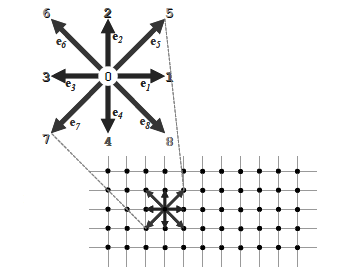
\includegraphics[height=4cm]{D2Q9_Grid.png}
    \caption{Example}
    \label{example_fig}
  \end{figure}
\end{frame}

\begin{frame}
  \frametitle{Lattice Arrangements}
  \framesubtitle{Lattices}
  The most used lattices are:
  \begin{itemize}
    \item For 1D problems:
      \begin{itemize}
	\item D1Q2
	\item D1Q3
	\item D1Q5
      \end{itemize}
    \item For 2D problems:
      \begin{itemize}
	\item D2Q4
	\item D2Q5
	\item D2Q9
      \end{itemize}
    \item For 3D problems:
      \begin{itemize}
	\item D3Q15
	\item D3Q19
      \end{itemize}
  \end{itemize}
\end{frame}

\begin{frame}
  \frametitle{1D Lattice Arrangements}
  \framesubtitle{D1Q2}
  Maybe the most basic of the lattices
  \begin{figure}
    \centering
    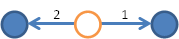
\includegraphics[height=1cm]{D1Q2.png}
    \caption{D1Q2}
  \end{figure}
  For this lattice, the velocity vectors are: $\vec{c_1}=1$ and $\vec{c_2}=-1$;
  the correspondent weighting factors are: $w_1=1/2$ and $w_2=1/2$;
  and the speed of sound in lattice ($\vec{C_s}$) is: $1/\sqrt{2}$.
\end{frame}

\begin{frame}
  \frametitle{1D Lattice Arrangements}
  \framesubtitle{D1Q3}
  \begin{figure}
    \centering
    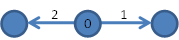
\includegraphics[height=1cm]{D1Q3.png}
    \caption{D1Q3}
  \end{figure}
  For this lattice, the velocity vectors are: $\vec{c_1}=1$, 
  $\vec{c_0}=0$  and $\vec{c_2}=-1$;
  the correspondent weighting factors are: $w_1=1/6$, $w_0=4/6$ and $w_2=1/6$;
  and the speed of sound in lattice ($\vec{C_s}$) is: $1/\sqrt{3}$.
\end{frame}

\begin{frame}
  \frametitle{1D Lattice Arrangements}
  \framesubtitle{D1Q5}
  \begin{figure}
    \centering
    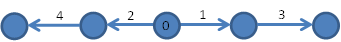
\includegraphics[height=1cm]{D1Q5.png}
    \caption{D1Q5}
  \end{figure}
  For this lattice, the velocity vectors are: $\vec{c_0}=0$, 
  $\vec{c_1}=1$, $\vec{c_2}=-1$, 
  $\vec{c_3}=2$ and $\vec{c_4}=-2$;
  the correspondent weighting factors are: $w_0=6/12$, $w_1=1/12$, 
  $w_2=1/12$, $w_3=2/12$ and $w_4=2/12$; and the speed of sound in lattice 
  ($\vec{C_s}$) is: $1/\sqrt{3}$.
\end{frame}

\begin{frame}
  \frametitle{2D Lattice Arrangements}
  \framesubtitle{D2Q4}
  \begin{figure}
    \centering
    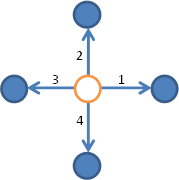
\includegraphics[height=2cm]{D2Q4.png}
    \caption{D2Q4}
  \end{figure}
  For this lattice, the velocity vectors are: $\vec{c_0}=(0,1)$, 
  $\vec{c_2}=(1,0)$, $\vec{c_3}=(0,-1)$ and 
  $\vec{c_4}=(-1,0)$; the correspondent weighting factors are: 
  $w_1=w_2=w_3=w_4=1/4$.
\end{frame}

\begin{frame}
  \frametitle{2D Lattice Arrangements}
  \framesubtitle{D2Q5}
  \begin{figure}
    \centering
    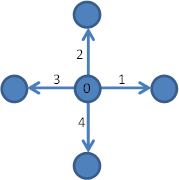
\includegraphics[height=2cm]{D2Q5.png}
    \caption{D2Q5}
  \end{figure}
  For this lattice, the velocity vectors are: $\vec{c_0}=(0,0)$, 
  $\vec{c_0}=(0,1)$, $\vec{c_2}=(1,0)$, 
  $\vec{c_3}=(0,-1)$ and $\vec{c_4}=(-1,0)$;
  the correspondent weighting factors are: $w_0=2/6$ and $w_1=w_2=w_3=w_4=1/6$.
\end{frame}

\begin{frame}
  \frametitle{2D Lattice Arrangements}
  \framesubtitle{D2Q9}
  \begin{figure}
    \centering
    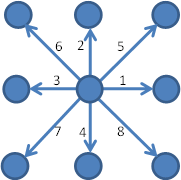
\includegraphics[height=2cm]{D2Q9.png}
    \caption{D2Q9}
  \end{figure}
    For this lattice, the velocity vectors are: $\vec{c_0}=(0,0)$, 
  $\vec{c_1}=(0,1)$, $\vec{c_2}=(1,0)$, 
  $\vec{c_3}=(0,-1)$, $\vec{c_4}=(-1,0)$, 
  $\vec{c_5}=(1,1)$, $\vec{c_6}=(-1,1)$, 
  $\vec{c_7}=(-1,-1)$ and $\vec{c_8}=(1,-1)$;
  the correspondent weighting factors are: $w_0=4/9$, $w_1=w_2=w_3=w_4=1/9$ 
  and $w_5=w_6=w_7=w_8=1/36$.
\end{frame}

\begin{frame}
  \frametitle{3D Lattice Arrangements}
  \framesubtitle{D3Q15}
  \begin{figure}
    \centering
    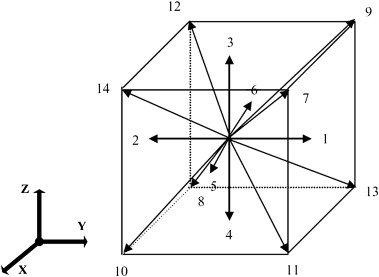
\includegraphics[height=3cm]{D3Q15.jpg}
    \caption{D3Q15}
  \end{figure}
    We can now figure out how the velocity vectors for any DnQm Lattice, 
  therefore so the only information that we need to specify every time is 
  the correspondent weighting factors: for $w_0=16/72$, 
  for $w_1$ to $w_6$ is $8/72$ and for $w_7$ to $w_14$ is $1/72$.
\end{frame}

\begin{frame}
  \frametitle{3D Lattice Arrangements}
  \framesubtitle{D3Q19}
  \begin{figure}
    \centering
    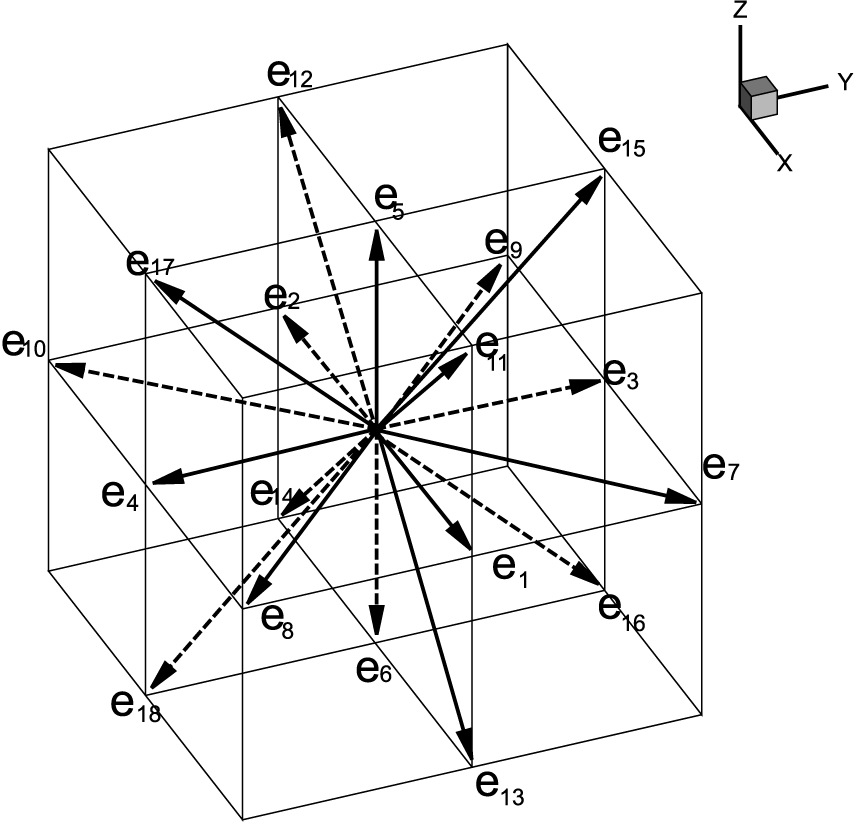
\includegraphics[height=3cm]{D3Q19.png}
    \caption{D3Q19}
  \end{figure}
    We can now figure out how the velocity vectors for any DnQm Lattice, 
  therefore so the only information that we need to specify every time is 
  the correspondent weighting factors: for $w_0=12/36$, 
  for $w_1$ to $w_6$ is $2/36$ and for $w_7$ to $w_18$ is $1/36$.
\end{frame}

\begin{frame}
  \frametitle{Equilibrium distribution Function}
  \framesubtitle{key to implemente LBM}

The key element in appyling LBM for different problems is the equilibrium distribution function, $f^{eq}$. 

We start from the normalized Maxwell's Distribution Function:
  \begin{equation}
   f = \frac{\rho}{2\pi/3} e^{-\frac{3}{2}(\vec{c}-\vec{u})^2} 
  \end{equation}
which can be written as,
  \begin{equation}
   f = \frac{\rho}{2\pi/3} e^{-\frac{3}{2}(c^2)}e^{(2\vec{c}.\vec{u} - u^2/2)}
  \end{equation}
where $ c^2 = \vec{c} \cdot \vec{c} $ and $ u^2 = \vec{u} \cdot \vec{u} $.
Recall that Taylor series expansion for $ e^{-x} $ is,
  \begin{equation}
   e^{-x} = 1 - x + \frac{x^2}{2!} - \frac{x^3}{3!} ...
  \end{equation}
\end{frame}

\begin{frame}
  \frametitle{Equilibrium distribution Function}
  \framesubtitle{key to implemente LBM}

Thefore the general equilibrium distribution can be writen as,
  \begin{equation}
   f = \frac{\rho}{2\pi/3} e^{-\frac{3}{2}(c^2)}[1+3(\vec{c} \cdot \vec{u})-\frac{3}{2} u^2 +...]
  \end{equation}
And the general from of the equilibrium distribution function can be written as,
  \begin{equation}
   f_i^{eq}=\phi\omega_i[A + B\vec{c}_i\cdot\vec{u}+ C(\vec{c}\cdot\vec{u})^2+ Du^2]
  \end{equation}
\end{frame}

\section{FDM vs LBM}

\begin{frame}
  \frametitle{The Lattice Boltzmann Method}
  \framesubtitle{by comparinson}
First let's use a simple case: A 1-D Diffusion Equation:
  \begin{equation}
   \frac{\partial T}{\partial t} = \alpha\frac{\partial^2 T}{\partial x^2}
  \end{equation}
and we are about to solve it by two methods:
  \begin{itemize}
    \item by Finite Difference Method (FDM)
    \item by Lattice Boltzmann Method (LBM)
  \end{itemize}
\end{frame}

\begin{frame}
  \frametitle{Finite Difference Approach}
  \framesubtitle{Using a uniform grid}
  Using a central difference in time and a second order central difference in space we get:
  \begin{equation}
   \frac{T_i^{n+1}-T_i^{n}}{\Delta t} = \alpha \frac{T_{i+1}^n-2T_i^n+T_{i-1}^n}{\Delta x^2}
  \end{equation}
  rearranging the above equation we get,
  \begin{equation}
    T_i^{n+1}-T_i^{n} = \frac{\alpha\Delta t}{{\Delta x^2}} T_{i+1}^n-2T_i^n+T_{i-1}^n
  \end{equation}
  and can be reformulated as,
  \begin{equation}
   T_i^{n+1}=T_i^{n} \left ( 1-\frac{\alpha\Delta t}{{\Delta x^2}} \right ) + \left (\frac{\alpha\Delta t}{{\Delta x^2}} \right ) \frac{T_{i+1}^n+T_{i-1}^n}{2}
  \end{equation}
\end{frame}

\begin{frame}
  \frametitle{Finite Difference Approach}
  \framesubtitle{Using a uniform grid}

  Now let 
  \begin{equation}
   \omega = \frac{2\alpha \Delta t}{\Delta x^2}
  \end{equation}

  Then our difference equation can be rewriten as;
  \begin{alertblock}{Important equation}
  \begin{equation}
   T_i^{n+1}=T_i^{n} \left (1 - \omega \right ) + \omega \frac{1}{2} \left ( T_{i+1}^n+T_{i-1}^n \right )
  \end{equation} 
  \end{alertblock}
\end{frame}

\begin{frame}
  \frametitle{using the LBM approach}
  \framesubtitle{using a D1Q2 lattices}
  \begin{block}{Start form the Boltzmann Equation}
  The kinetic equation for the distribution function (Temperature distribution, 
  species distribution, etc), $f_k(x,t)$ can be written as:
  \begin{equation} \nonumber
    \frac{\partial f_k(x,t))}{\partial t}+c_k \frac{\partial f_k(x,t))}{\partial x} = \Omega_k
  \end{equation} 
  for i=1,2 (for our one dimensional problem)
  \end{block}
  The left hand side term represents the streaming process, where the distribution 
  function streams (advects along the lattice link with velocity
  $c_k=\frac{\Delta x}{\Delta t}$.
\end{frame}

\begin{frame}
  \frametitle{using the LBM approach}
  \framesubtitle{using a D1Q2 lattices}
  using the BGK approximation for the collision operator:
  \begin{equation} \nonumber
   \Omega_k = -\frac{1}{\tau}[f_k(x,t)-f_k^{eq}(x,t)]
  \end{equation}
  The kinetic lattice boltzmann can be discretized as,
  \begin{eqnarray}
   && \frac{f_k(x,t+\Delta t))- f_k(x,y)}{\Delta t} + \nonumber \\
   && c_k\cdot\frac{f_k(x+\Delta x,t+\Delta t)- f_k(x,t+\Delta t)}{\Delta x} \nonumber \\
   && = -\frac{1}{\tau}[f_k(x,t)-f_k^{eq}(x,t)] 
  \end{eqnarray}
  Note that $\Delta x = c_k \Delta t$
\end{frame}

\begin{frame}
  \frametitle{using the LBM approach}
  \framesubtitle{using a D1Q2 lattices}
  This would leads again to:
  \begin{equation} \nonumber
    f_k(x+\Delta x,t+\Delta t)-f_k(x,t)=-\frac{\Delta t}{\tau}[f_k(x,t)-f_k^{eq}(x,t)] 
  \end{equation}
  if we do $\omega = \Delta t/ \tau$ and re-arrange the variables as:
  \begin{alertblock}{Do it looks familiar?}
  \begin{equation} \nonumber
   f_k(x+\Delta x,t+\Delta t) = f_k(x,t)\left(1-\omega\right) + \omega\frac{1}{2} \left(f_k^{eq}\right)
  \end{equation}
  \end{alertblock}
  This equation is the working horse of our diffusion problem and it represents 
  a set of equations for each of the linkages of our lattice.
\end{frame}

\begin{frame}
  \frametitle{using the LBM approach}
  \framesubtitle{using a D1Q2 lattices}
  for our case the dependent variable $T(x,t)$ can be related to the distribution function $f_k$ as:
  \begin{equation}
   T(x,t) = \sum_{k=1}^{2} f_k(x,t)
  \end{equation}
  and the equilibrium distribution can be choosen as $f_k^{eq} =$ $w_k T(x,t)$ where $w_k$ is 
  the weighting factor in the direction of each linkage.
\end{frame}

\begin{frame}
  \frametitle{using the LBM approach}
  \framesubtitle{using a D1Q2 lattices}
  We must remember that the weighting factor shoud sum 1, $\sum_{k=1}^{2} w_k = 1$ and the equilibrium
  distribution can be assumed valid along al k-directions,
  \begin{equation}
    T(x,t)=\sum_{k=1}^{2} f_k^{eq}(x,t)=\sum_{k=1}^{2} w_k T(x,t)
  \end{equation}
  The relation between $\alpha$ and $\omega$ can be reduced from multi-scale expansion by using 
  chapmann-Enskog expansion, which yield:
  \begin{equation}
    \alpha = \frac{\Delta x^2}{\Delta t D}(\tau - \frac{1}{2})
  \end{equation}
  where D is the dimension of the problem, 1, 2 or 3.
\end{frame}

\begin{frame}
  \frametitle{using the LBM approach}
  \framesubtitle{using a D1Q2 lattices}
  Now we must define our Equilibrium function:
  Recall equation (12):
  \begin{equation} \nonumber
    f_i^{eq}=T(x,t) w_i[A + B\vec{c}_i\cdot\vec{u}+ C(\vec{c}\cdot\vec{u})^2+ Du^2]
  \end{equation}
  it is appropiate that the equilibrium function be assumed constant, 
  where no macroscopic velocity is involved, let:
  \begin{equation}
    f_i^{eq}=A_i
  \end{equation}
\end{frame}

\begin{frame}
  \frametitle{using the LBM approach}
  \framesubtitle{using a D1Q2 lattices}
  and it must satisfy:
  \begin{eqnarray}
    && \sum_{i=1}^{2}f_k^{eq}=T(x,t) \\
    && \sum_{i=1}^{2}f_k^{eq}c_k=0
  \end{eqnarray}
which leads to the equations:
  \begin{eqnarray}
    && A_1+A_2 = T(x,t) \\
    && A_1 c_1+A_2 c_2 = 0
  \end{eqnarray}
\end{frame}

\begin{frame}
  \frametitle{using the LBM approach}
  \framesubtitle{using a D1Q2 lattices}
  but we know that $c_1 = 1$ and $c_2 = -1$, which leads us to
  \begin{eqnarray}
    && A_1+A_2 = T(x,t) \\
    && A_1-A_2 = 0 \mapsto A_1=A_2
  \end{eqnarray}
  thus $A_1$ = $A_2$ = T(x,t)/2 or $f_k^{eq} = 1/2 T(x,t)$
\end{frame}

\section{1D Case}

\begin{frame}
  \frametitle{1D Diffusion Case}
  \framesubtitle{Using LBM D1Q2}
  A slab initially at temperature equal to zero, $T=0$. For time $t\ge0$, the left surface 
  of the slab is subjected to a high temperature and equal to unity, $T=1$. The slab length 
  is 30 units. Calculate the temperature distribution in the slab for t=200. Compare the 
  of both methods, LBM and FDM, for $\alpha=25$.
  \begin{figure}
    \centering
    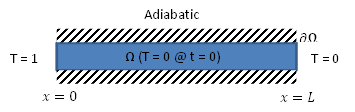
\includegraphics[height=2cm]{Heat_Problem_1D.png}
  \end{figure}
\end{frame}

\begin{frame}
  \frametitle{1D Diffusion Case}
  \framesubtitle{Using LBM D1Q2}
  Solution:
  Let us devide the domain of integration into $\Delta x = 1.0$ and $\Delta t= 1.0$
  using $\alpha = 0.25$ we can compute $\omega : 0.25 = (1/\omega-1/2)$ with gives 
  $\omega = 4/3$.
  
  we know from the equilibrium function analysis that for D1Q2, de equilibrium function
  is,
  \begin{eqnarray}
    && f_1^{eq}(x,t)=0.5T(x,t)\\
    && f_2^{eq}(x,t)=0.5T(x,t)
  \end{eqnarray}
  LBM consist of two steps, collision and streaming.
  The collision step is given by:
  \begin{equation} \nonumber
    f_k^{eq}(x,t+\Delta t)=f_k(x,t)[1-\omega]+\omega f_k^{eq}(x,t)
  \end{equation}
  And the Streaming step is:
  \begin{equation} \nonumber
    f_k(x+\Delta x,t+\Delta t)= f_k(x,t+\Delta t)
  \end{equation}
\end{frame}

\begin{frame}
  \frametitle{1D Diffusion Case}
  \framesubtitle{Boundary Conditions}
  The boundary conditions for LBM are obtained by contrasting the macroscopic 
  conditions with the streaming process near the boundaries. For our case we would use:
    \begin{itemize}
     \item Dirichlet Boundary Conditions.
     \item Neumann Boundary Conditions.
    \end{itemize}

\end{frame}

\begin{frame}
  \frametitle{1D Diffusion Case}
  \framesubtitle{Boundary Conditions}
  \begin{itemize}
     \item Dirichlet Boundary Condition
    \end{itemize}
  The detailed flux balance at the boundary, x=o for D1Q2 is as follows,
  \begin{equation} \nonumber
   f_q^eq(0,t)-f_1(0,t)+f^{eq}-f_2(0,t)=0
  \end{equation}
  and,
  \begin{eqnarray} \nonumber
    && f_1^{eq}(0,t)=w_1 T_w = 0.5T_w \\
    && f_2^{eq}(0,t)=w_2 T_w = 0.5T_w
  \end{eqnarray}
  Therefore at $x=0$, $f_1(0)+f_2(0) = T_w$, and from the streaming processes 
  $f_1(0)=f_2(1)$, then $f_1(0)$ can be determined as $f_1(0)=T_w-f_2(0)$.
\end{frame}


\begin{frame}
  \frametitle{1D Diffusion Case}
  \framesubtitle{Boundary Conditions}
    \begin{itemize}
     \item Neumann Boundary Condition
    \end{itemize}
  The temperature gradient is zero which implies that at x = n, $T(n)= T(n-1)$.
  Hence,
  \begin{equation} \nonumber
    f_1(n)+f_2(n)=f_1(n-1)+f_2(n-1)
  \end{equation}
  or 
  \begin{eqnarray} 
    && f_1(n)=f_1(n-1) \nonumber \\
    && f_2(n)=f_2(n-1) \nonumber
  \end{eqnarray}
  where $n$ denotes the lattice node.
\end{frame}

\begin{frame}
  \frametitle{1D Diffusion Case}
  \framesubtitle{Result using D1Q2}
  The result of our algorithm should be:
  \begin{figure}
    \centering
    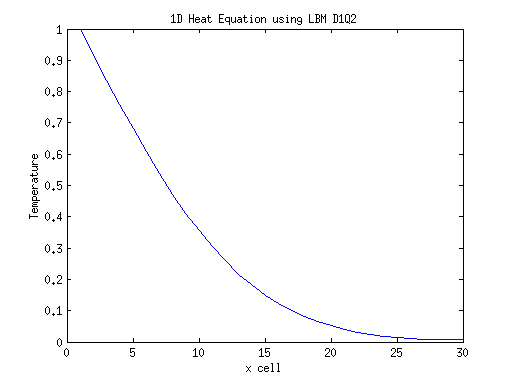
\includegraphics[height=5cm]{heat_eq_d1q2.png}
  \end{figure}
\end{frame}

\begin{frame}
  \frametitle{1D Diffusion Case}
  \framesubtitle{Result using FDM}
  The result of our algorithm should be:
  \begin{figure}
    \centering
    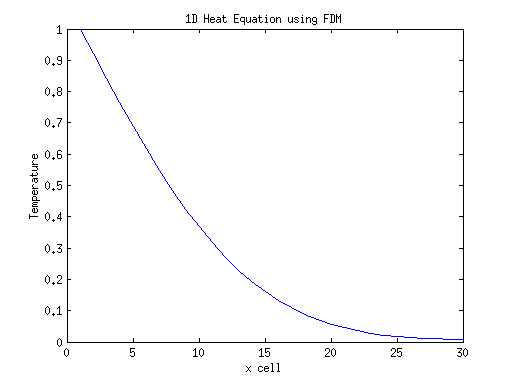
\includegraphics[height=5cm]{heat_eq_fdm.png}
  \end{figure}
\end{frame}

\section{More Examples}

\begin{frame}
  \frametitle{2D Diffusion Case}
  \framesubtitle{Result using D2Q4}

  \begin{figure}
    \centering
    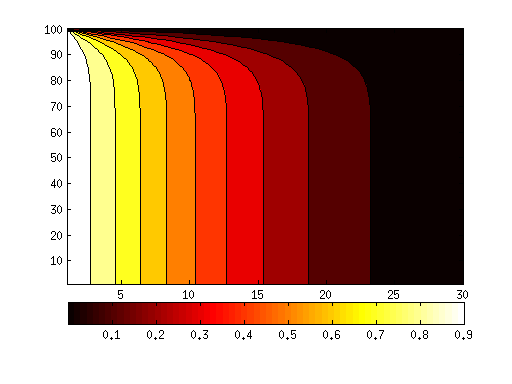
\includegraphics[height=5cm]{heat_eq_d2q4.png}
  \end{figure}

\end{frame}

\begin{frame}
  \frametitle{1D Advection-Diffusion Case}
  \framesubtitle{Result using D1Q2}

  \begin{figure}
    \centering
    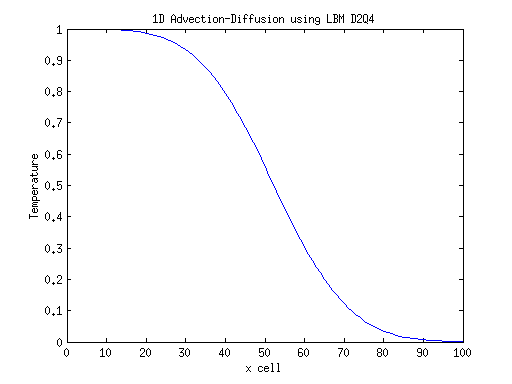
\includegraphics[height=5cm]{advec_diff_d1q2.png}
  \end{figure}
\end{frame}

\begin{frame}
  \frametitle{2D Advection-Diffusion Case}
  \framesubtitle{Result using D2Q4}

  \begin{figure}
    \centering
    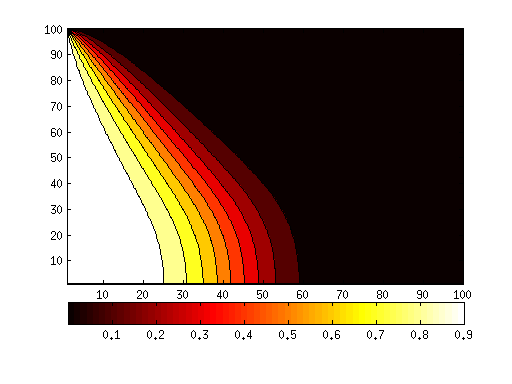
\includegraphics[height=5cm]{advec_diff_d2q4.png}
  \end{figure}

\end{frame}

%\begin{frame}
%  \frametitle{Ideal Case}
%  \framesubtitle{Result using D2Q9}

%  \begin{figure}
%    \centering
%    \includegraphics[height=5cm]{advec_diff_d2q9.png}
%  \end{figure}

%\end{frame}


\begin{frame}
  \frametitle{Resources}
  \framesubtitle{If you want to have more details on LBM}
  \begin{thebibliography}{10}

  \beamertemplatearticlebibitems

  \bibitem{A short introduction to LBM}
    Anne Hanna, ``A short intro to LBM''
    \newblock {\tt http://icarusswims.blogspot.com/2011/04/}

  \bibitem{Lattice Bolzmann Method}
    A.A. Mohamad, ``Lattice Boltzmann Method''
    \newblock {\tt http://www.springer.com/engineering/}

  \bibitem{The Lattice Bolzmann Equation}
    Sauro Succi, ``The Lattice Boltzmann Equation''
    \newblock {\tt Oxford University Press}

  \end{thebibliography}
\end{frame}

\frame{
  \vspace{2cm}
  {\huge Questions ?}

  \vspace{3cm}
  \begin{flushright}
    Aerodynamics and Analysis Lab

    \structure{\footnotesize{manuel.ade@gmail.com}}
  \end{flushright}
}

\end{document}
